\documentclass[11pt]{beamer}
\usetheme{Goettingen}
\usepackage[utf8]{inputenc}
\usepackage{amsmath}
\usepackage{amsfonts}
\usepackage{amssymb}
\usepackage{graphicx}
\usepackage{hyperref}
\author{Alex Heilman}
\title{NV-Centers in Diamond as a Qubit Platform}
\subtitle{An Overview}
%\setbeamercovered{transparent} 
%\setbeamertemplate{navigation symbols}{} 
%\logo{} 
%\institute{} 
%\date{} 
%\subject{} 

\newenvironment{boxed2}
    {\begin{center}
    \begin{tabular}{|p{0.95\textwidth}|}
    \hline\\
    }
    { 
    \\\\\hline
    \end{tabular} 
    \end{center}
    }


\begin{document}

\begin{frame}
\titlepage
\end{frame}

%\begin{frame}
%\tableofcontents
%\end{frame}

\begin{frame}{Overview}

$\bullet$ What's a qubit? \pause What can be a qubit?

\vspace{1cm}\pause

$\bullet$ What's an NV Center?

\vspace{1cm}\pause

$\bullet$ How is an NV Center a qubit?

\vspace{1cm}\pause

\end{frame}

\section{Qubit Criteria}
\begin{frame}{What's a Qubit?}


I think we've seen this plenty of times\pause , in case you haven't:

\vspace{.7cm}

\begin{center}
Two-level Quantum System:


$$
\vert 0 \rangle = \begin{bmatrix}
1 \\ 0
\end{bmatrix} \quad\ \ \vert 1 \rangle = \begin{bmatrix}
0 \\ 1
\end{bmatrix}
$$

$$
\vert \psi \rangle = \alpha \vert 0 \rangle + \beta \vert 1 \rangle
$$

$$
\text{Normalized: }\alpha^2 +\beta^2 = 1
$$

\pause

\vspace{0.4cm}

What criteria for physical systems do we need to satisfy?
\end{center}

\end{frame}

\begin{frame}{Criteria for Qubit Platforms}

\begin{boxed2}
\textbf{DiVincenzo's Criteria:} The first five are for quantum computers.

$\bullet$ Scalable and discernible

\medskip

$\bullet$ Fiduciary initial state

\medskip

$\bullet$ Long decoherence time

\medskip

$\bullet$ Universal gate set

\medskip

$\bullet$ Measureable

\medskip

These next two are for quantum communication

\medskip

$\bullet$ Memory $\rightarrow$ Computation

\medskip

$\bullet$ Faithful transmission


\end{boxed2}
\end{frame}

\begin{frame}{Criteria for Qubit Platforms cont.}

Let's just focus on a few here:\pause

\vspace{1cm}

$\bullet$ Initialization

\vspace{1cm}\pause

$\bullet$ Control

\vspace{1cm}\pause

$\bullet$ Measurement

\vspace{1cm}\pause

$\bullet$ Coherence Time

\end{frame}


\section{Defects in Diamond}
\begin{frame}{Why Defects?}
Defects can give us localized electronic and spin states trapped in a solid state system.

\vspace{.8cm}\pause

Also, gives us more prospective systems, since for every solid state system we'll have (atleast) a few possible defects

\vspace{.8cm}\pause

Really, the concepts discussed below should apply to most similar systems, it's just that this system is well-studied and has convenient energy levels/properties
\end{frame}

\begin{frame}{Why Diamond?}
Diamond is an ideal candidate due to low density of phonon modes (relatively high Debye temperature)

\begin{center}

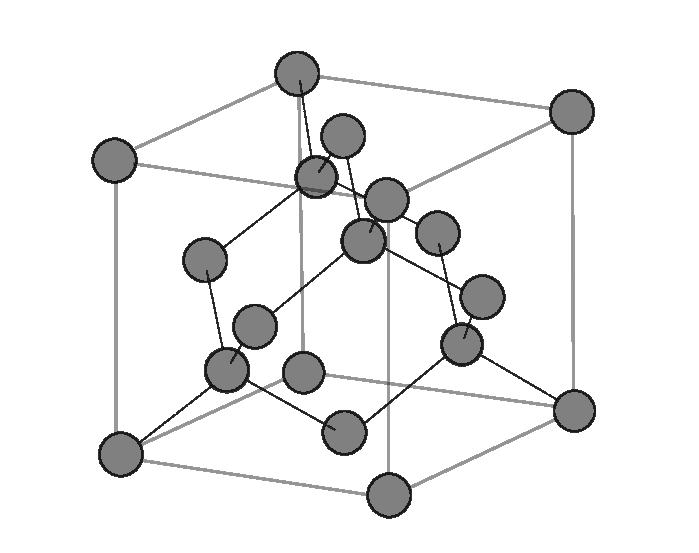
\includegraphics[scale=0.47]{diamond_uc.pdf}

\end{center}\pause

This leaves spins of defects and electrons less influenced by phonon modes, increasing their coherence times
\end{frame}

\begin{frame}{What's an NV-Center}
NV-Center refers to a type of defect in diamond lattices with several charge states (-, +, neutral). \pause The most commonly discussed charge state is the (-) NV-Center. If unspecified, this is most likely the defect under consideration.


\vspace{5cm}

\end{frame}

\begin{frame}{What's an (-) NV-Center}
An (-) NV-Center is a neighboring nitrogen-vacancy defect in diamond with an extra electron %(completes the neighboring carbon's valence shell)

\begin{center}

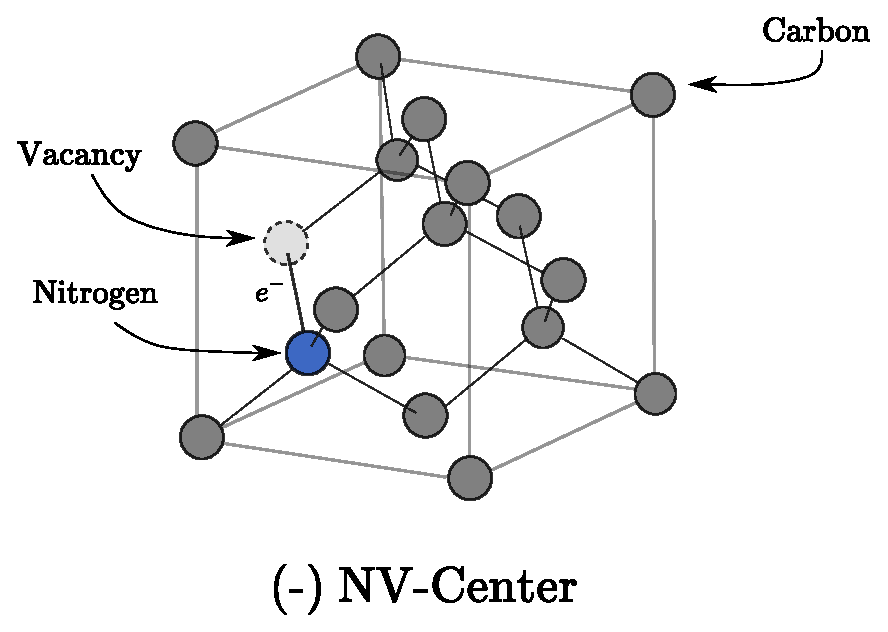
\includegraphics[scale=0.43]{diamond_nv.pdf}

\end{center}\pause

This results in a 'center' between the two with localized energy/spin  states.\pause

\medskip

These energy states may be used as a Qubit platform.

\end{frame}
\subsection{Hamiltonian}
\begin{frame}{Spin Hamiltonian Effects}
We're really interested in the spin state of the electron. \pause
Primarily dependent on spin-spin and spin-magnetic field interactions (we'll ignore electric fields here); with the relevant effects being:

\vspace{.7cm}\pause

(Electron State) Zero-Field Splitting (ZFS): $SDS$

\vspace{.7cm}\pause

(Nuclear Spin) Quadrapole Interaction: $IQI$ 

\vspace{.7cm}\pause

(Spin-Spin) Hyper-fine Interactions:  $SAI$

\vspace{.7cm}\pause

(Spin-B Field) Zeeman: $g_sSB, g_iI_iB$ \pause $\leftarrow$ This we can control!

\medskip\pause

\begin{center}
Let's see the Hamiltonian...
\end{center}
\end{frame}

\begin{frame}{NV-Center Hamiltonian}
The electron will be taken to be localized to the defect. We'll take this localized two electron state to be the unperturbed solution and apply some interaction effects, with the corresponding interaction Hamiltonian below (again, assuming no external electric field/Stark effects):
\begin{align*}
H&=\underbrace{\vec{\hat{S}}\mathbf{D}\vec{\hat{S}}}_{\text{ZFS}} +   \underbrace{\vec{\hat{I}}_N\mathbf{Q} \vec{\hat{I}}_N}_{\text{Quadrapole}}+\underbrace{\vec{\hat{S}}\big(\mathbf{A}_N\vec{\hat{I_N}}+\sum_i\mathbf{A}_{C_i}\vec{\hat{I}}_{C_i}\big)}_{\text{Hyperfine}}\\
&\quad +\underbrace{\big(\vec{\hat{S}}\mathbf{g}_s+\vec{\hat{I}}_N\mathbf{g}_N+\sum_i\vec{\hat{I}}_{C_i}\mathbf{g}_{C_i}\big)\vec{B}}_{\text{Zeeman}}\quad\cite{gali2019ab}\\
\end{align*}
%&\quad +\underbrace{\big(\vec{\hat{}}\mathbf{g}_s+\vec{\hat{I}}_N\mathbf{g}_N+\sum_i\vec{\hat{I}}_{C_i}\mathbf{g}_{C_i}\big)\vec{E}}_{\text{Stark}}\\
\end{frame}
\subsection{Simplifications}
\begin{frame}{Simplifications}
Assuming we apply a magnetic field only along the symmetry axis, which we define to be the $z$ direction\pause ; and neglecting the surrounding carbon's effects(both Zeeman and hyperfine, though these allow us to use the nv-center as register for these surrounding sites \cite{PhysRevX.9.031045}):\pause
$$
H_{NV}\approx DS_z^2 + \omega_eS_z + QI_z^2 +\omega_nI_z + AS_zI_z\quad\cite{PhysRevLett.129.100501}
$$
where $\omega_i = \gamma_i B$, the Larmor frequency. 

$D=2\pi\times (2.87 GHz)$, the dipole coupling constant

$Q=2\pi\times (-4.95 GHz)$, the nuclear quadrapole coupling constant

$A=2\pi\times (-2.16 GHz)$, the hyperfine coupling constant

%Assume $S_x=S_y$ along center's axis so E=0 for ZFS, other tensors become diagonal for chosen coordinates and B-field orientation
\end{frame}
\subsection{Energy Levels}
\begin{frame}{Energy Levels}
\begin{center}
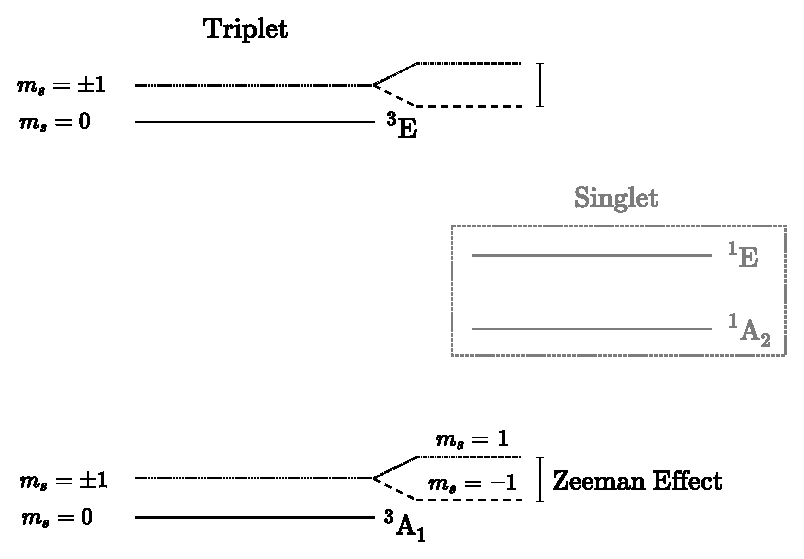
\includegraphics[scale=0.76]{energy_raw.pdf}
\end{center}
\vspace{0.7cm}
\end{frame}

\section{NV as Qubit}

\begin{frame}{Qubit States}
The localized spin states of the defect may be used as a two-level system.\pause

\vspace{.4cm}

We make the identifications:

\begin{center}
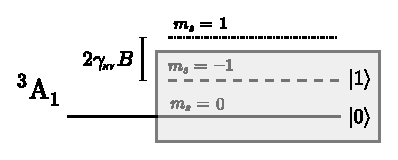
\includegraphics[scale=1.3]{energy_qubit.pdf}
\end{center}\pause

The transitions between these states are in the microwave regime.
\end{frame}

\subsection{Initialization}
\begin{frame}{Initialization}
\small
Initialization to the zero state can be achieved by an asymmetric relaxation from the first excited triplet state ($^3E$) to the triplet ground state ($^3A$).


\begin{center}
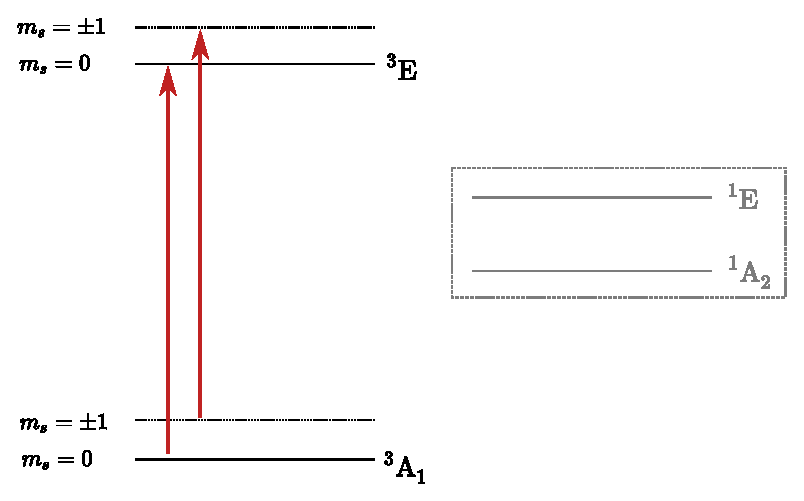
\includegraphics[scale=0.6]{energy_init.pdf}
\end{center}

Applying a resonant pulse (532 nm) excites all triplet ground states to their corresponding excited states ($\Delta m_s=0$).
\end{frame}

\begin{frame}{Initialization cont.}\small

Excited $m_s=0$ states have been shown to decay back into $m_s=0$ ground states, but $m_s=\pm 1$ excited states favor a non-radiative (vibrational) decay mode via the singlet states, back into the $m_s=0$ ground state.

\begin{center}
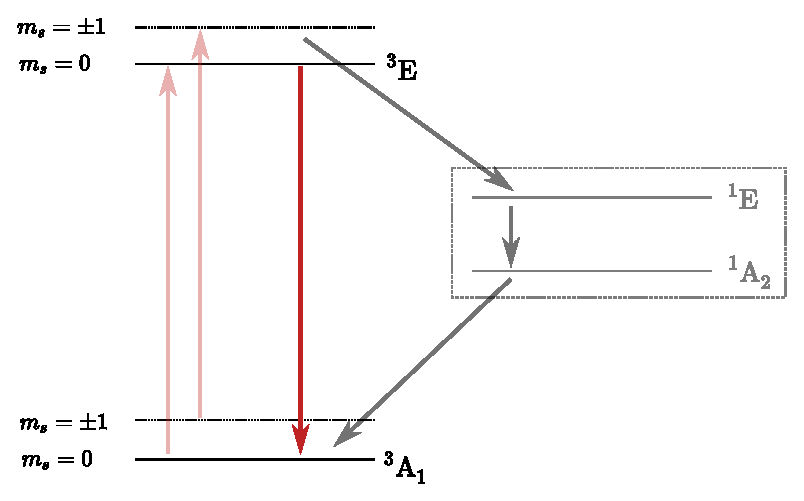
\includegraphics[scale=0.6]{energy_init_relax.pdf}
\end{center}

This may be exploited to intialize the spin state into our $\vert 0 \rangle$ state.
\end{frame}

\subsection{Gates}
\begin{frame}{Local Control}
Perpendicular (polarization relative symmetry axis) microwave pulses can induce Rabi flopping of state between $\vert 0 \rangle$ and $\vert 1 \rangle$ 

\begin{center}
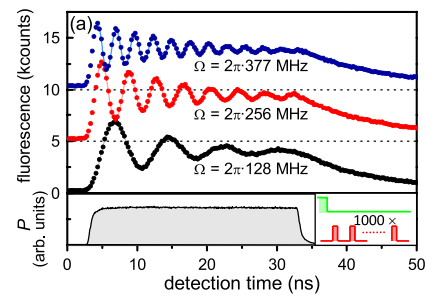
\includegraphics[scale=1]{rabi.png} $\ \ $ \cite{PhysRevLett.105.177403}
\end{center}


\end{frame}

%\begin{frame}{Entangling Operations}
%Spin-photon coupling then photon-photon state entanglement+measurement of photons may result in entangled pair of spins.
%\end{frame}

\subsection{Measurement}
\begin{frame}{Optically Detected Magnetic Resonance}\small
Much like the initialization technique, optically detected magnetic resonance (ODMR) takes advantage of the asymmetric relaxation modes of the excited state.

\begin{center}
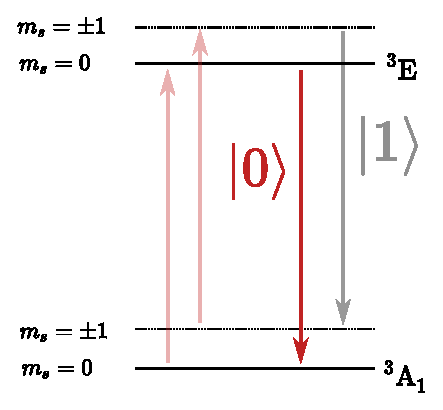
\includegraphics[scale=0.6]{energy_measure.pdf}
\end{center}

Hence, if the defect flouresces when hit with a resonant pulse, it was measured to be in the $\vert 0 \rangle$ state, but if it's 'dark' after a resonant pulse, it can be considered to have been in the $\vert 1 \rangle$ state.

\medskip


\end{frame}

\begin{frame}{Measurement Cont.}
Note also that these allows our read-out to essentially be part of the next computation's initialization.

\vspace{.5cm}\pause

One problem, however, is the possibility of internal reflection of the emitted photon. \pause This can be solved with an immersion lens built into the diamond \cite{hadden2010strongly}.
\end{frame}

\section*{ }
\begin{frame}{Conclusion \& Outlook}

Promising candidate due to practical methods of initialization, measurement, and qubit manipulation. 

\medskip\pause

Long coherence times, room temperature stability

\medskip\pause

Haven't discussed scalability, two (or more) qubit operations, quantum networking, etc.

\medskip\pause

Recent works have used neighboring spins (of carbon and nitrogen) as additional qubits \cite{PhysRevX.9.031045} or used spin-photon coupling to get distant centers to interact \cite{nemoto2016photonic}

\medskip\pause

Some have also considered defect levels as qutrits \cite{PhysRevLett.129.100501}

\end{frame}

\begin{frame}[allowframebreaks]{References}
\bibliographystyle{plain}

\bibliography{nv} 

\end{frame}
\end{document}